\documentclass[tikz]{standalone}

\usepackage{pgf}
\usepackage{tikz}
\usetikzlibrary{calc}
\usetikzlibrary{shadows}
\usetikzlibrary{arrows}
\usetikzlibrary{positioning}
\usetikzlibrary{shapes}
\usetikzlibrary{shadows}
\usetikzlibrary{3d}
\usetikzlibrary{arrows}
\usetikzlibrary{decorations.pathreplacing}

\begin{document}



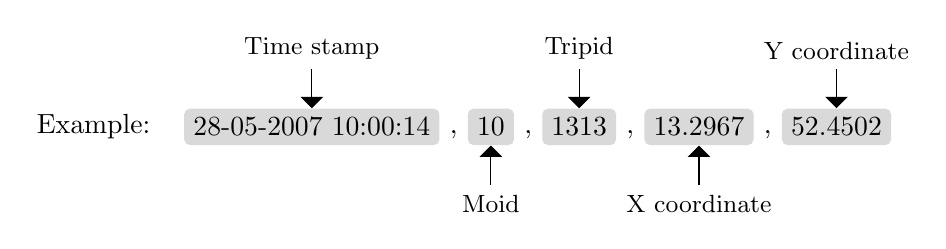
\begin{tikzpicture}[scale=1,  every node/.style={transform shape, anchor=base west}]

\node (t0) {Example:};
\node[fill=gray!30,anchor=base, rounded corners=2pt, right=3mm of t0] (t1) {28-05-2007 10:00:14};
\node[anchor=base,right=0mm of t1] (t2) {,\vphantom{10:00:14}};
\node[fill=gray!30,anchor=base, rounded corners=2pt, right=0mm of t2] (t3) {10};
\node[anchor=base,right=0mm of t3] (t4) {,\vphantom{10:00:14}};
\node[fill=gray!30,anchor=base, rounded corners=2pt, right=0mm of t4] (t5) {1313};    
\node[anchor=base,right=0mm of t5] (t6) {,\vphantom{10:00:14}};
\node[fill=gray!30,anchor=base, rounded corners=2pt, right=0mm of t6] (t7) {13.2967};    
\node[anchor=base,right=0mm of t7] (t8) {,\vphantom{10:00:14}};
\node[fill=gray!30,anchor=base, rounded corners=2pt, right=0mm of t8] (t9) {52.4502};    

\node[above=5mm of t1] (e1) {\small Time stamp};
\node[below=5mm of t3] (e2) {\small Moid};
\node[above=5mm of t5] (e3) {\small Tripid};
\node[below=5mm of t7] (e4) {\small X coordinate};
\node[above=5mm of t9] (e5) {\small Y coordinate};

\path[-triangle 90, draw](e1) -- (t1);
\path[-triangle 90, draw](e2) -- (t3);
\path[-triangle 90, draw](e3) -- (t5);
\path[-triangle 90, draw](e4) -- (t7);
\path[-triangle 90, draw](e5) -- (t9);
\end{tikzpicture}

\end{document}



